\documentclass[useAMS, usenatbib, a4paper]{mnras}
\pdfsuppresswarningpagegroup=1
\usepackage[spanish,es-minimal,english]{babel}
\usepackage[utf8]{inputenc}
\usepackage{graphicx}
\let\Bbbk\relax
\usepackage{amsmath}	% Advanced maths commands
\usepackage{amssymb}	% Extra maths symbols
\usepackage{xcolor}
\usepackage{fixltx2e}
\usepackage{hyperref}
\usepackage{savesym}
\savesymbol{tablenum}
\usepackage{siunitx}
\restoresymbol{SIX}{tablenum}
\usepackage{newtxtext}
\usepackage[varg,varvw,smallerops]{newtxmath}
\usepackage{xfrac} % for the \sfrac macro
\usepackage{booktabs}
\usepackage{longtable}
\usepackage{array}   % for \newcolumntype macro
\newcolumntype{L}{>{$}l<{$}} % math-mode version of lrc column types
\newcolumntype{R}{>{$}r<{$}} 
\newcolumntype{C}{>{$}c<{$}}
\hypersetup{colorlinks=True, linkcolor=blue!50!black, citecolor=black,
  urlcolor=blue!50!black}
\usepackage{etoolbox}
\robustify\bfseries
\robustify\itshape
\usepackage{enumerate}
\bibliographystyle{mnras}
\sisetup{
  % explicit""+" is useful for velocities
  retain-explicit-plus = true,
  % prefer 10^6 over 1 x 10^6
  retain-unity-mantissa = false,
  % Use x +/- e instead of x(e)  
  separate-uncertainty = true,
  % Make sure to pick up bold font when used in section heading for instance
  detect-weight = true,
  table-align-uncertainty = true,
  table-align-comparator = true,
}
\DeclareSIUnit\msun{\text{M\ensuremath{_\odot}}}
\DeclareSIUnit\lsun{\text{L\ensuremath{_\odot}}}
\DeclareSIUnit\zsun{\text{Z\ensuremath{_\odot}}}
\DeclareSIUnit\angstrom{\text{\AA}}

% A better \ion command that works in more circumstances
\newcommand\ION[2]{#1\,\scalebox{0.9}[0.8]{\uppercase{#2}}}
\newcounter{ionstage}
\renewcommand{\ion}[2]{\setcounter{ionstage}{#2}% 
  \ensuremath{\mathrm{#1\,\scriptstyle\Roman{ionstage}}}}
\newcommand\hii{\ion{H}{2}}

% Alternative title: Scaling laws for turbulent H II regions
\title[Scaling laws for turbulent H II regions]
{
  % Turbulence-driven temperature fluctuations in H II regions
  Scaling laws for turbulent H II regions
}

\author[Henney et al.]{
  William J. Henney\textsuperscript{1}\thanks{w.henney@irya.unam.mx},
  J. García-Vázquez\textsuperscript{2},
  S. J. Arthur\textsuperscript{1},
  Sac-Nicté X. Medina\textsuperscript{3},
  and others?
  \\
  \textsuperscript{1}\foreignlanguage{spanish}{%
    Instituto de Radioastronomía y
    Astrofísica, Universidad Nacional Autónoma de México, Apartado
    Postal 3-72, 58090 Morelia, Michoacán, Mexico}\\
  \textsuperscript{2}\foreignlanguage{spanish}{%
    Escuela Superior de Física y Matemáticas,
    Instituto Politécnico Nacional,
    U.P. Adolfo López Mateos, Zacatenco,
    Ciudad de México, México C.P. 07738}\\
  \textsuperscript{3}German Aerospace Center,
  Scientific Information, 51147, Cologne, Germany;
  Max-Planck-Institut für Radioastronomie, Auf dem Hügel 69, 53121, Bonn, Germany\\
}


% These dates will be filled out by the publisher
\date{Accepted XXX. Received YYY; in original form ZZZ}

% Enter the current year, for the copyright statements etc.
\pubyear{2024}


\begin{document}
\label{firstpage}
\pagerange{\pageref{firstpage}--\pageref{lastpage}}
\maketitle



\begin{abstract}
Turbulence can cause temperature fluctuations via two mechanisms in \hii{} regions, via a direct mechanism, and by an indirect mechanism. In the direct mechanism, dissipation of the turbulent kinetic energy acts as a fluctuating heating source for the gas. In the indirect mechanism, the shocks cause density fluctuations, which modulate the ionizing flux that arrives at the outer parts of the \hii{} region, causing the boundary to move in and out, transitioning between a recombination front and an ionization front. If the modulation timescale corresponds to the recombination timescale, then a portion of the gas is out of thermal equilibrium.
\end{abstract}

\begin{keywords}
HII regions -- ISM: kinematics and dynamics -- turbulence 
\end{keywords}
%\facilities{VLT:Yepun (MUSE); OANSPM:2.1m (Mezcal); Keck (HIRES)}
%\object{M42}

\section{Introduction}
\label{sec:introduction}
\begin{figure*}
  \centering
  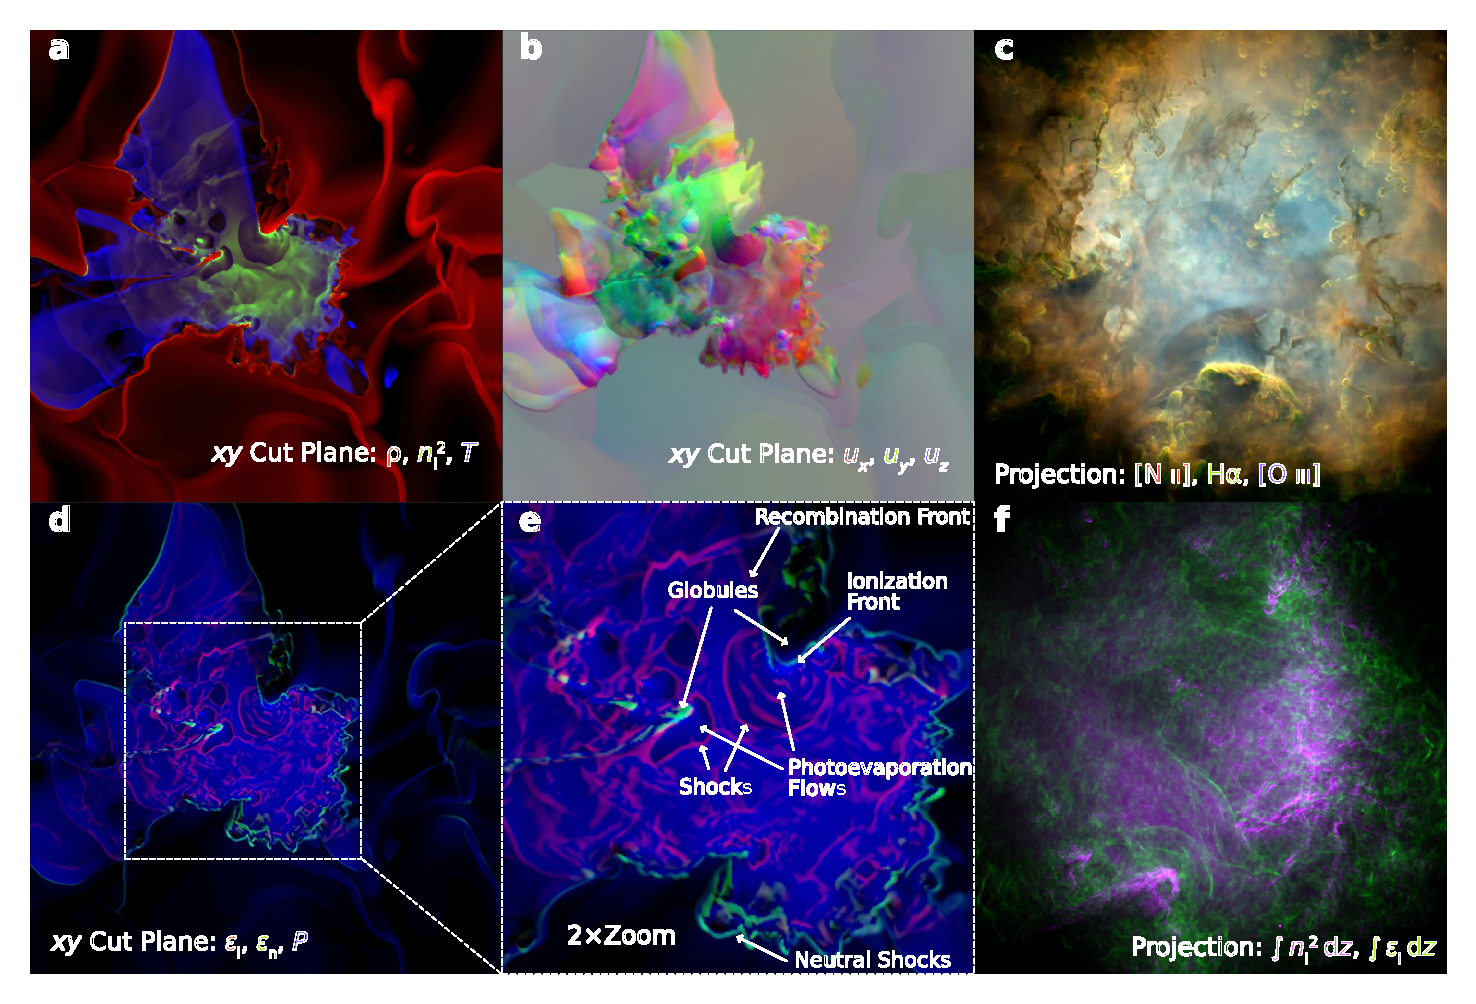
\includegraphics[width=\linewidth]{figs/kb512-ke-diss-multipanel}
  \caption{Structure of a single-star \hii{} region
    from a three-dimensional radiation-hydrodynamics simulation \citep{medina2014}.
    (a) Plane \(xy\) cut through the fields of gas density (red), squared ionized density (green), and gas temperature (blue).
    (b) Vector velocity field for the same cut: red, green, blue show \(u_x\), \(u_y\), \(u_z\),
    with dark colors indicating negative values and light colors positive values. Mid gray indicates zero.
    (c) Simulated surface brightness image of the simulation cube in 3 different optical emission lines:      
}
  \label{fig:kb512-mosaic}
\end{figure*}


There are reasons to be suspicious of the high temperatures in ionization transition zones
seen in Figure~\ref{fig:kb512-mosaic}a.
The non-local effects of the diffuse ionizing radiation field
are not considered in the simulation
and the atomic physics of the heating and cooling processes are treated in a very approximate way \citep{Henney:2009b}. 

\section{Summary of García-Vázquez et al. (2023)}
\label{sec:summary-garcia}



\section*{Data availability statement}
\label{sec:data-avail-stat}
All data and accompanying analysis programs used in this paper are available
from the github repository \url{https://github.com/will-henney/turb-t2-paper}.

\bibliography{turb-t2-refs}
\appendix
\section{Cloudy models of low-velocity shocks in \hii{} regions}
\label{sec:cloudy-models-low}



% Don't change these lines
\bsp	% typesetting comment
\label{lastpage}

\end{document}

%%% Local Variables:
%%% mode: LaTeX
%%% TeX-master: t
%%% End:
